
\chapter{Implementacija i korisničko sučelje}

	
		
		\section{Korištene tehnologije i alati}

        Timsku komunikaciju smo uspješno ostvarili kroz aplikaciju \href{https://discord.com/}{Discord}, pružajući jednostavnu i iznimno organiziranu interakciju putem "channel" i "thread" opcija. Za izradu UML dijagrama smo koristili alat \href{https://astah.net/products/astah-uml/}{Astah UML}, dok smo za upravljanje izvornim kodom primijenili \href{https://github.com/}{GitHub}.

        Kao razvojno okruženje odabrali smo \href{https://www.jetbrains.com/idea/}{IntelliJ IDEA}, integrirano razvojno okruženje (IDE) tvrtke JetBrains. Ovo okruženje pruža napredne mogućnosti kao što su dovršavanje koda analizom konteksta, navigacija koda s mogućnošću izravnog skakanja na klasu ili deklaraciju u kodu, refaktoriranje koda, rješavanje pogrešaka te ugrađene naredbe za Git, uz mnogobrojna proširenja za različite programske jezike i alate.

        Na strani klijentske aplikacije (frontend), koristili smo \href{https://reactjs.org/}{React.js}, popularnu \href{https://www.javascript.com/}{JavaScript} biblioteku za izradu korisničkih sučelja u web aplikacijama. Virtualna DOM tehnologija ovog okvira doprinosi efikasnijem ažuriranju sučelja, unaprjeđujući performanse i korisničko iskustvo.

        Za poslužiteljsku stranu aplikacije (backend) odabrali smo \href{https://spring.io/}{Spring Framework}, sveobuhvatan okvir za \href{https://www.java.com/en/}{Java} programski jezik. Poznat po konceptima inverzije kontrole i ubrizgavanja ovisnosti, Spring olakšava razvoj aplikacija pružajući modularnost, testabilnost te olakšava održavanje koda. Za upravljanje bazama podataka koristili smo \href{https://www.postgresql.org/}{PostgreSQL}, moćan objektno-relacijski sustav otvorenog koda. Njegova pouzdanost, skalabilnost i podrška za kompleksne upite čine ga optimalnim izborom za naše potrebe.
			
			\eject
		
	
		\section{Ispitivanje programskog rješenja}
			

			
			\subsection{Ispitivanje komponenti}

			 Provedbu ispitivanja implementiranih funkcionalnosti proveli smo na razini komponenti kroz detaljne unit testove. Fokusirali smo se na provjeru ispravnosti pomo- ćnih funkcija koje su ključne u različitim dijelovima koda. Ukupno smo izvršili sedam testova, a u nastavku donosimo sažete opise svakog testa zajedno s pripadajućim kodovima. Svaki opis testa popraćen je slikom koja jasno prikazuje rezultate izvođenja. Ovaj pristup omogućio nam je temeljitu analizu osnovne funkcionalnosti i identifikaciju rubnih uvjeta, pridonoseći sigurnosti i stabilnosti cijelog sustava. Nastojali smo osigurati sveobuhvatan pregled implementiranih funkcionalnosti kroz precizno definirane ispitne slučajeve.


            \subsubsection{Ispitni slučaj 1.: Test provjere svojstva dokumenta}

                        \noindent\textbf{Ulaz:}
                        \begin{packed_item}
                        	\item  Stvaranje primjerka korisnika (User) i postavljanje njegovih svojstava (ID i nadimak)
                        	\item  Stvaranje primjerka dokumenta (Document) i postavljanje njegovih svojstava (ID korisnika, korisnik, status dokumenta).
                        \end{packed_item}

                        \noindent\textbf{Očekivani rezultati:}
                        \begin{packed_item}
                        	\item  Očekujemo da će dokument imati ispravno postavljene vrijednosti svojstava, u skladu s postavljenim ulaznim podacima.
                        \end{packed_item}
                      
                        \noindent\textbf{Rezultat:}
                        \begin{packed_item}
                        	\item  Izvršavanje ovog dijela testa provjerava ispravnost postavljanja svojstava dokumenta i uspoređuje ih s očekivanim rezultatima.
                        \end{packed_item}
                       \begin{figure} [H]
                       	\centering
                       	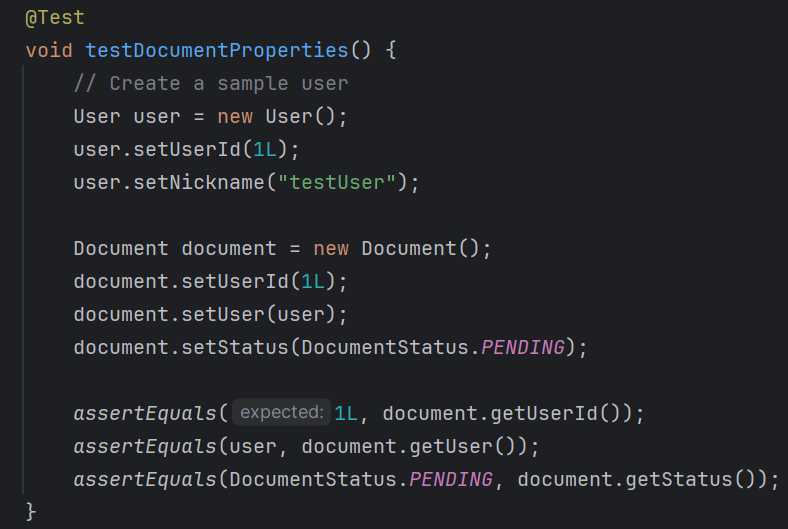
\includegraphics[width=0.7\linewidth]{slike/DokumentTest.png}
                       	\caption{Test provjere svojstva dokumenta}
                       	\label{fig:Test provjere svojstva dokumenta}
                       \end{figure}
                      



            \subsubsection{Ispitni slučaj 2.: Test provjere funkcionalnosti ImageChangeRequestStatus}

                                    \noindent\textbf{Ulaz:}
                                    \begin{packed_item}
                                    	\item Nema posebnog ulaza jer testira vrijednosti unutar samog enuma
                                    \end{packed_item}
                      
                                    \noindent\textbf{Očekivani rezultati:}
                                    \begin{packed_item}
                                    	\item Očekujemo da će vrijednosti enuma biti ispravno postavljene.
                                    	\item Očekujemo da će konverzija enuma u String biti ispravna.
                                    \end{packed_item}
                                    \noindent\textbf{Rezultat:}
                                    \begin{packed_item}
                                    	\item Izvršavanje testa provjerava da li su vrijednosti enuma ImageChangeRequestStatus ispravno postavljene
                                    	\item Izvršavanje testa provjerava da li su vrijednosti enuma ImageChangeRequestStatus ispravno postavljene
                                    \end{packed_item}
                                    
                                    
                        \begin{figure} [H]
                        	\centering
                        	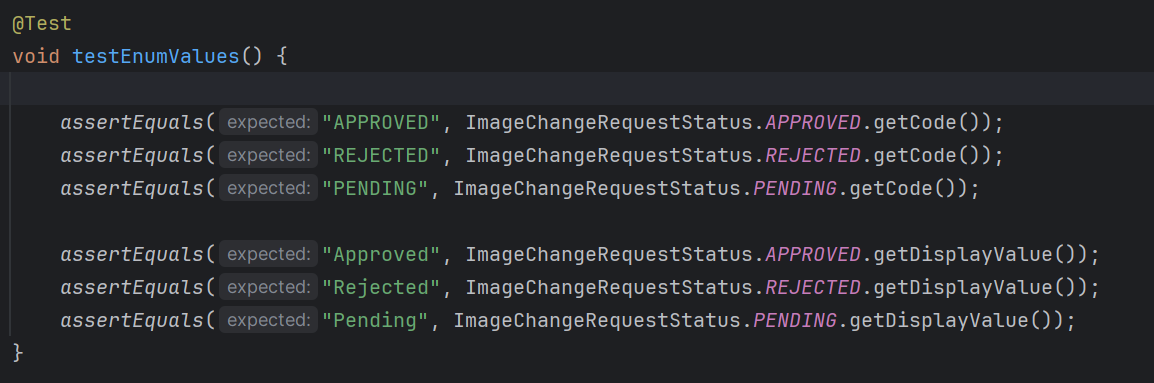
\includegraphics[width=0.7\linewidth]{slike/ImageChangeTest.png}
                        	\caption{Test provjere funkcionalnosti ImageChangeRequestStatus}
                        	\label{fig:Test provjere funkcionalnosti ImageChangeRequestStatus}
                        \end{figure}
                        
                        \begin{figure} [H]
                        	\centering
                        	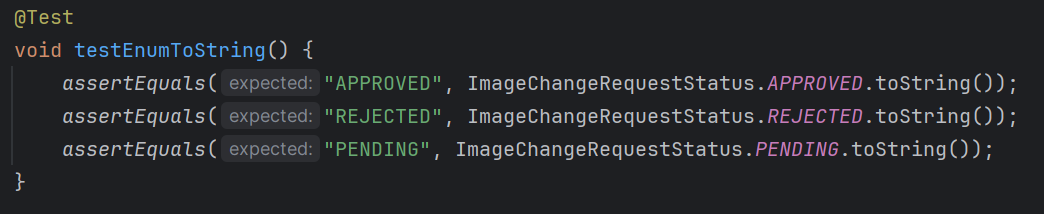
\includegraphics[width=0.7\linewidth]{slike/ImageChangeTest1.png}
                        	\caption{Test provjere funkcionalnosti ImageChangeRequestStatus}
                        	\label{fig:Test provjere funkcionalnosti ImageChangeRequestStatus}
                        \end{figure}
                                    
      

			\subsubsection{Ispitni slučaj 3.: Provjera vraćanja vremena u razredu Listing}
					\noindent\textbf{Ulaz:}
					\begin{packed_item}
						\item Stvaranje instance razreda Listing
						\item Postavljanje vremena povratka (returnByTime) na trenutno vrijeme
					\end{packed_item}
					
					\noindent\textbf{Očekivani rezultati:}
					\begin{packed_item}
						\item Očekujemo da će vrijeme povratka biti jednako trenutnom vremenu u obliku Timestamp objekta
						\item Očekujemo da će vrijednost vremena povratka biti null, budući da nije postavljena
					\end{packed_item}
					 \noindent\textbf{Rezultat:}
					\begin{packed_item}
						\item  Izvršavanje testa provjerava postavljanje i dohvaćanje vremena povratka, uspo- ređujući ga s očekivanim rezultatom
						\item  Izvršavanje testa provjerava da li je vrijednost vremena povratka null, što ukazuje na ispravno ponašanje u slučaju ne postavljanja vremena povratka
					\end{packed_item}
					
					 \begin{figure} [H]
						\centering
						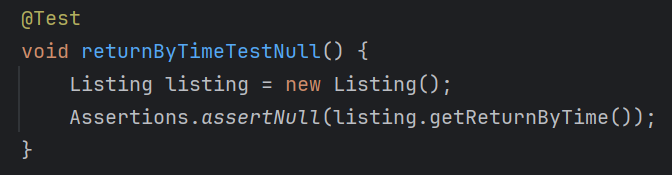
\includegraphics[width=0.7\linewidth]{slike/ListingTest.png}
						\caption{Provjera vraćanja vremena u razredu Listing}
						\label{fig:Provjera vraćanja vremena u razredu Listing}
					\end{figure}
					 \begin{figure} [H]
						\centering
						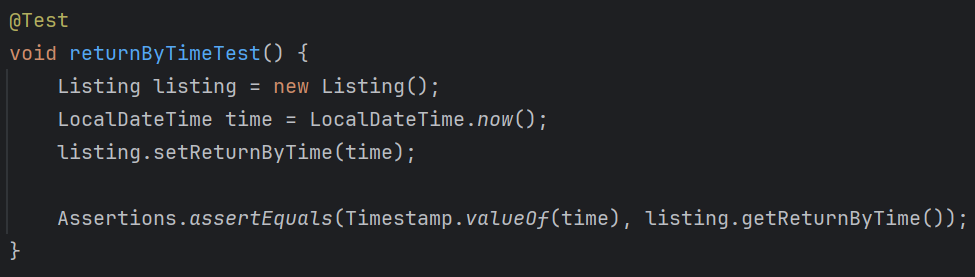
\includegraphics[width=0.7\linewidth]{slike/ListingTest1.png}
						\caption{Provjera vraćanja vremena u razredu Listing}
						\label{fig:Provjera vraćanja vremena u razredu Listing}
					\end{figure}


			\subsubsection{Ispitni slučaj 4.: Test provjere svojstava skutera}

					\noindent\textbf{Ulaz:}
					\begin{packed_item}
						\item Stvaranje primjerka korisnika (User) i postavljanje njegovih svojstava (ID i nadimak)
						\item Stvaranje primjerka skutera (Scooter) i postavljanje njegovih svojstava (ID, proizvođač, model, kapacitet baterije, maksimalna brzina, putanja do slike, maksimalni doseg, godina proizvodnje, dodatne informacije, korisnik, dostupnost)
					\end{packed_item}
					
					\noindent\textbf{Očekivani rezultati:}
					\begin{packed_item}
						\item Očekujemo da će svojstva skutera biti ispravno postavljena prema unesenim vrijednostima.
					\end{packed_item}
					\noindent\textbf{Rezultat:}
					\begin{packed_item}
						\item  Izvršavanje testa provjerava ispravnost postavljanja svojstava skutera i uspo- ređuje ih s očekivanim rezultatima.
						 postavljanja vremena povratka
					\end{packed_item}
              \begin{figure} [H]
              	\centering
              	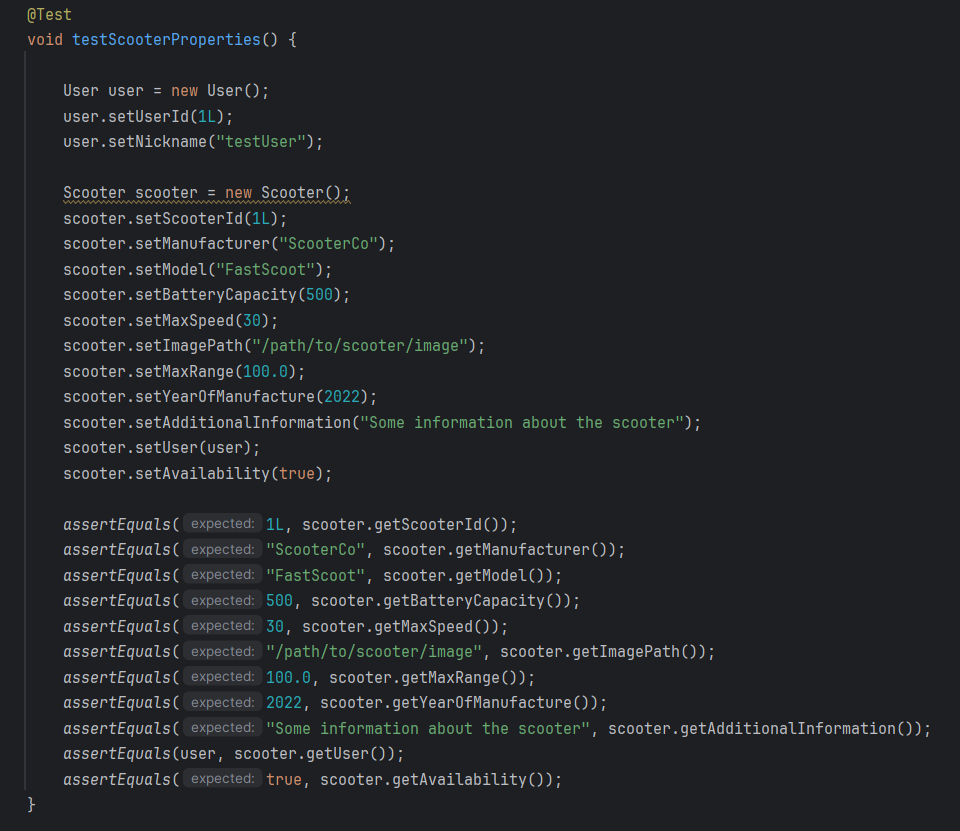
\includegraphics[width=0.7\linewidth]{slike/ScooterTest.png}
              	\caption{Test provjere svojstava skutera}
              	\label{fig:Test provjere svojstava skutera}
              \end{figure}

     
			\subsubsection{Ispitni slučaj 5.: Test provjere vremena plaćanja u razredu transakcije}
			
			
			\noindent \textbf{Ulaz:}
			\begin{packed_item}
				\item Stvaranje instance razreda Transaction
				\item Postavljanje vremena plaćanja (paymentTime) na trenutno vrijeme
			\end{packed_item}
			
			\noindent \textbf{Očekivani rezultati:}
			\begin{packed_item}
				\item Očekujemo da će vrijeme plaćanja biti jednako trenutnom vremenu u obliku Timestamp objekta
				\item Očekujemo da će vrijednost vremena plaćanja biti null, budući da nije postavljena
			\end{packed_item}
			\noindent \textbf{Rezultat:}
			\begin{packed_item}
				\item  Izvršavanje testa provjerava postavljanje i dohvaćanje vremena plaćanja, uspo- ređujući ga s očekivanim rezultatom
				\item Izvršavanje testa provjerava da li je vrijednost vremena plaćanja null, što ukazuje na ispravno ponašanje u slučaju ne postavljanja vremena plaćanja.
			\end{packed_item}
			
			\begin{figure} [H]
				\centering
				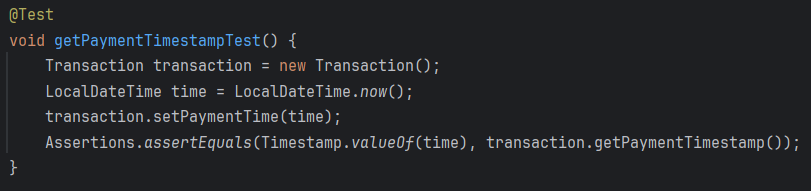
\includegraphics[width=0.7\linewidth]{slike/TransactionTest.png}
				\caption{Test provjere vremena plaćanja u razredu transakcije}
				\label{fig:Test provjere vremena plaćanja u razredu transakcije}
			\end{figure}
			\begin{figure} [H]
				\centering
				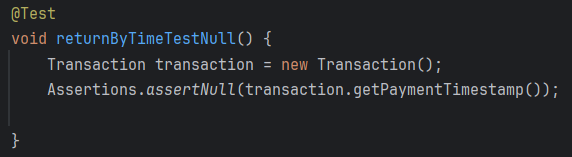
\includegraphics[width=0.7\linewidth]{slike/TransactionTest1.png}
				\caption{Test provjere vremena plaćanja u razredu transakcije}
				\label{fig:Test provjere vremena plaćanja u razredu transakcije}
			\end{figure}

                                                                      
           


            \subsubsection{Ispitni slučaj 6.: Test provjere svojstva korisnika}
            
            \noindent\textbf{Ulaz:}
            \begin{packed_item}
            	\item Stvaranje primjerka korisnika (User) i postavljanje njegovih svojstava (ID, nadimak, ime, prezime, broj kartice, e-mail, broj telefona, lozinka, uloga, status)
            \end{packed_item}
            
            \noindent\textbf{Očekivani rezultati:}
            \begin{packed_item}
            	\item Očekujemo da će svojstva korisnika biti ispravno postavljena prema unesenim vrijednostima
            \end{packed_item}
            \noindent\textbf{Rezultat:}
            \begin{packed_item}
            	\item  Izvršavanje testa provjerava ispravnost postavljanja svojstava korisnika i uspo- ređuje ih s očekivanim rezultatima
            \end{packed_item}

				\begin{figure} [H]
					\centering
					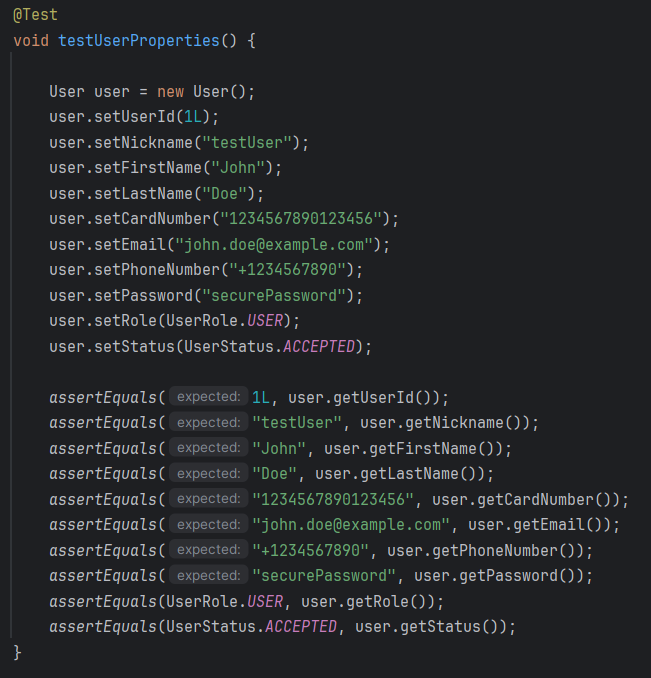
\includegraphics[width=0.7\linewidth]{slike/UserTest.png}
					\caption{Test provjere svojstva korisnika}
					\label{fig:Test provjere svojstva korisnika}
				\end{figure}

        


            \subsubsection{Ispitni slučaj 7.: Test provjere funkcionalnosti prijave korisnika}
            
             \noindent\textbf{Ulaz:}
            \begin{packed_item}
            	\item Koristi se Mock objekt UserRepository
            	\item Koristi se UserService objekt, gdje je userService injektiran u UserService pomoću @InjectMocks
            	\item Postavlja se Mock korisnik (mockUser) s podacima za prijavu
            \end{packed_item}
            
            \noindent\textbf{Očekivani rezultati:}
            \begin{packed_item}
            	\item Očekuje se da će korisničko ime i lozinka odgovarati podacima Mock korisnika
            	\item Očekuje se da će userService uspješno vratiti Mock korisnika
            	
            \end{packed_item}
            \noindent\textbf{Rezultat:}
            \begin{packed_item}
            	\item  Izvršava se prijava korisnika pomoću userService.login("test@example.com", "password")
            	\item  Provjerava se je li rezultat jednak Mock korisniku (mockUser)
            \end{packed_item}
				\begin{figure} [H]
					\centering
					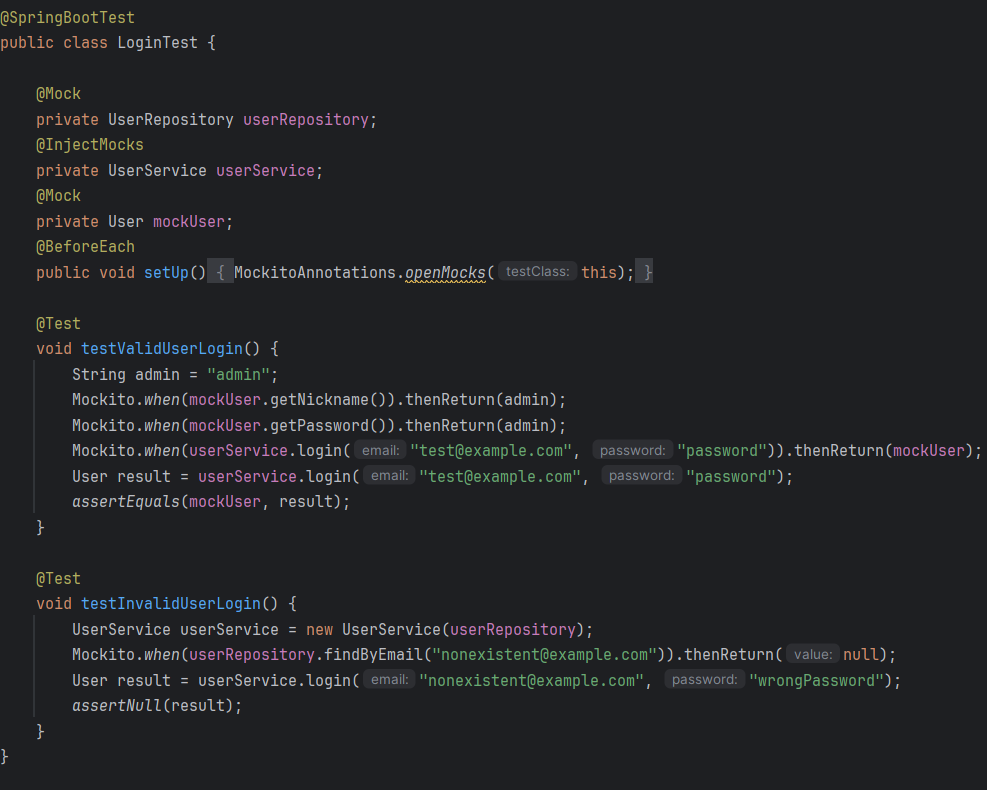
\includegraphics[width=0.7\linewidth]{slike/LoginTest.png}
					\caption{Test provjere funkcionalnosti prijave korisnika}
					\label{fig:Test provjere funkcionalnosti prijave korisnika}
				\end{figure}
                                                                                           
                       



			\subsection{Ispitivanje sustava}



			\subsubsection{Ispitni slučaj 1: Provjera ispravnosti registracije}
			
			\noindent\textbf{Cilj:}
			\begin{packed_item}
				Automatsko testiranje procesa registracije novog korisnika koji ne unese broj mobitela na web stranici pomoću Selenium WebDriver s Chrome preglednikom.
			\end{packed_item}
			
			\noindent\textbf{Koraci testiranja:}
			\begin{packed_item}
				\item Navigacija na stranicu za registraciju
				\item Ispunjavanje svih polja registracijskog obrazca osim polja za broj mobitela
				\item  Potvrda Registracije
				\item  Provjera je li se korisnik registrirao
				
			\end{packed_item}
			\noindent\textbf{Očekivani rezultati:}
			\begin{packed_item}
				\item  Korisnik se nije uspio registrirati
				\item Ispisana odgovarajuća poruka
			\end{packed_item}


						\begin{figure} [H]
							\centering
							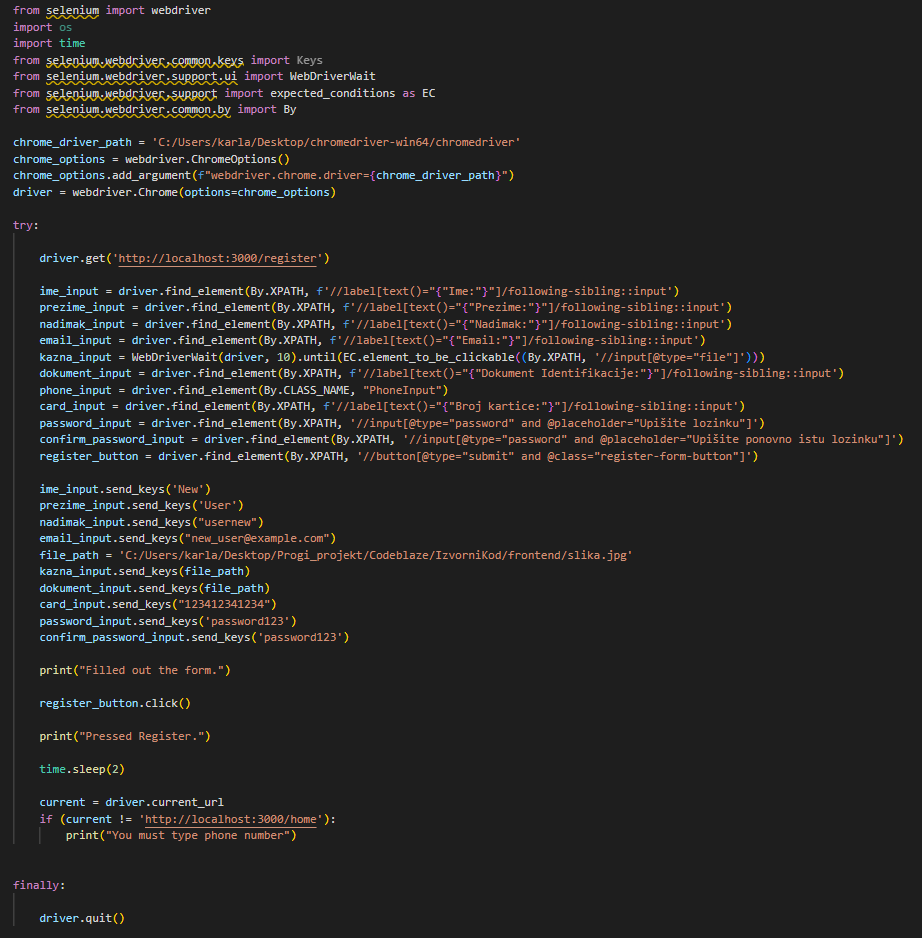
\includegraphics[width=0.7\linewidth]{slike/RegisterSelenium.png}
							\caption{Provjera ispravnosti registracije}
							\label{fig:Provjera ispravnosti registracije}
						\end{figure}
						
						\begin{figure} [H]
							\centering
							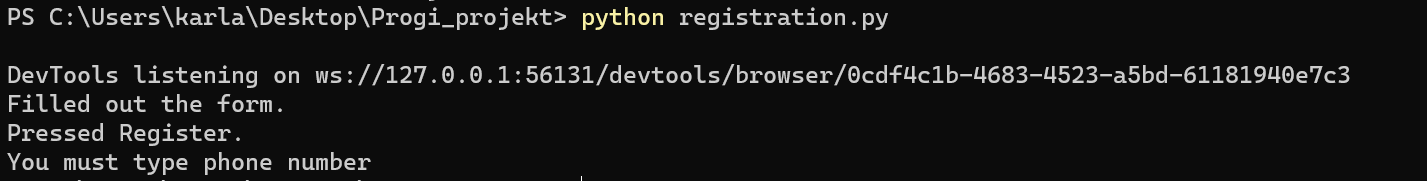
\includegraphics[width=0.7\linewidth]{slike/RegisterSeleniumOutput.png}
							\caption{Provjera ispravnosti registracije}
							\label{fig:Provjera ispravnosti registracije}
						\end{figure}

                        


            \subsubsection{Ispitni slučaj 2: Provjera ispravnosti prijave}

                        Ovaj Selenium test simulira korisničku prijavu na web stranici, unoseći korisničko ime i lozinku te provjerava očekivani rezultat, tj. naslov stranice nakon prijave.
                        
                        \noindent\textbf{Cilj:}
                        \begin{packed_item}
                        	Automatsko testiranje procesa prijavljivanja na web stranicu pomoću Selenium WebDriver s Chrome preglednikom.
                        \end{packed_item}
                        
                        \noindent\textbf{Koraci testiranja:}
                        \begin{packed_item}
                        	\item Navigacija na stranicu za prijavu
                        	\item  Unos podataka za prijavu
                        	\item Provjera stranice nakon prijave
                        	
                        \end{packed_item}
                        \noindent\textbf{Očekivani rezultati:}
                        \begin{packed_item}
                        	\item  Poruka "Assertion successful: 'Codeblaze' is in the title." ispisuje se kao potvrda uspješne prijave.
                        \end{packed_item}
                                                             

				\begin{figure} [H]
					\centering
					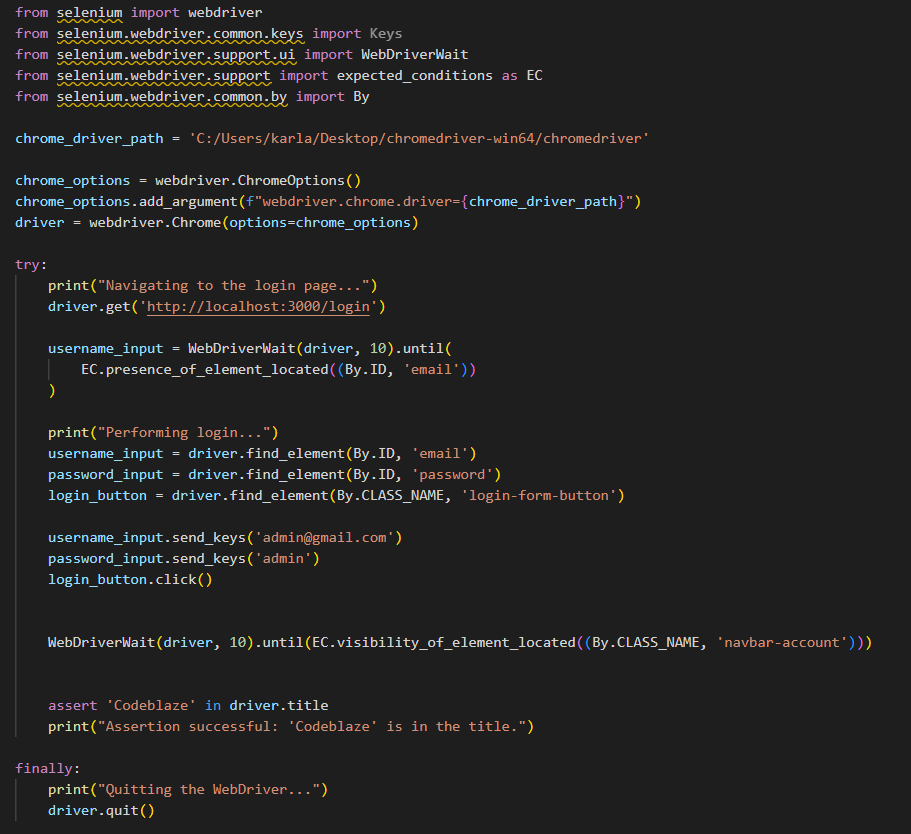
\includegraphics[width=0.7\linewidth]{slike/LoginSelenium.png}
					\caption{Provjera ispravnosti prijava}
					\label{fig:Provjera ispravnosti prijava}
				\end{figure}
				\begin{figure} [H]
					\centering
					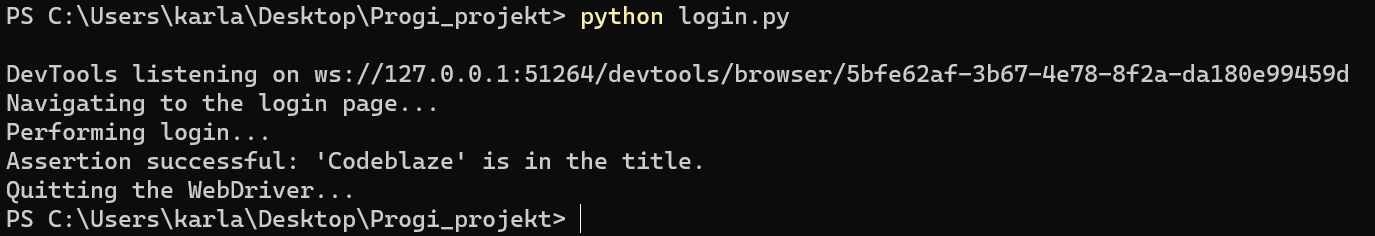
\includegraphics[width=0.7\linewidth]{slike/LoginSeleniumOutput.png}
					\caption{Provjera ispravnosti prijava}
					\label{fig:Provjera ispravnosti prijava}
				\end{figure}
                                  




			
			\eject 
		
		
		\section{Dijagram razmještaja}
			
			Dijagram rasporeda ilustrira kako su fizički i softverski resursi distribuirani unutar operativnog okvira sustava. Na serveru se smještaju dva ključna servisa: servis za web i servis za upravljanje bazom podataka. Kroz web preglednike, korisnici stječu pristup funkcionalnostima web aplikacije. Ovaj sustav funkcioniše po modelu klijent-server arhitekture gdje je komunikacijski protokol između korisničkih uređaja i servera omogućen putem HTTP veze.

		\begin{figure} [H]
			\centering
			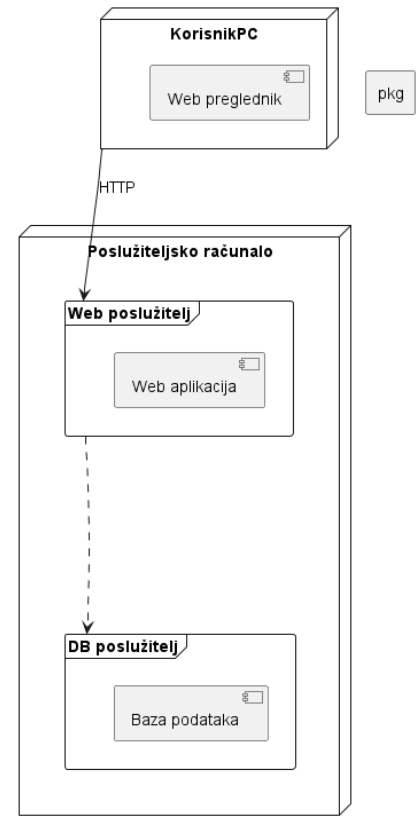
\includegraphics[width=0.7\linewidth]{dijagrami/dijagramRazmjestanja.png}
			\caption{Prikaz dijagrama razmještanja}
			\label{fig:Prikaz dijagrama razmještanja}
		\end{figure}

			\eject 
		
		\section{Upute za puštanje u pogon}

		Za postavljanje aplikacije u produkcijsko okruženje, ključno je implementirati sve komponente na GitHub platformi. Ovaj korak je presudan jer omogućava kreiranje Docker kontejnera, koji su esencijalni za funkcionalnost aplikacije u radnom okruženju. Izvorni kod naše aplikacije dostupan je na https://github.com/Kvesa- Fer/Codeblaze.

		Implementaciju aplikacije izvodimo kroz Render, cloud-based platformu-as-a-service (PaaS). Render nudi potrebnu infrastrukturu za pokretanje aplikacije. Prije početka rada na Render platformi, neophodno je u korijenskom direktoriju izvornog koda kreirati 'render.yaml' datoteku. Ova datoteka služi kao 'Blueprint spec', konfiguracijski set za implementaciju i aktivaciju aplikacije na Render platformi.

		U 'render.yaml' datoteci definiramo tri ključna servisa naše aplikacije: 'server', 'client', i 'db'. Svaki servis, osim PostgreSQL baze, treba sadržavati atribute 'type', 'name', i 'env'. Za PostgreSQL bazu, potrebno je navesti samo 'name', a detalji implementacije su već dostupni kroz predefiniranu uslugu na Render platformi.

		Dodatno, definiramo svojstva za preostale servise - frontend i backend. Atribut 'env' određuje okruženje izvođenja i postavljen je na 'Docker', što omogućava izgradnju aplikacije kroz Docker kontejnere. Svaki definirani servis predstavlja zasebnu 'Docker image' datoteku, koja uključuje kod, alate, biblioteke i ostale postavke potrebne za izgradnju kontejnera.

		Za svaki servis, 'repo' svojstvo postavljamo na putanju GitHub repozitorija s izvornim kodom aplikacije. Također, definiramo 'branch' svojstvo na 'main' granu i 'rootDir' za određivanje korijenskog direktorija repozitorija. 'BuildFilter' svojstvo omogućava definiranje putanje do datoteka čije promjene na 'main' grani iniciraju redeployment servisa.

		Za postavljanje varijabli okruženja, koristimo mogućnost definiranja zavisnosti varijabli jednog servisa o svojstvima već postojećih Render servisa. Varijable okru- ženja za 'backend' servis povezan s bazom podataka dohvaćamo preko definiranih svojstava Render servisa za PostgreSQL bazu. Ostale varijable, koje su privatne, postavljamo direktno na Render platformu.

		Kreiranje korisničkog računa i prijava na https://dashboard.render.com/ su prvi koraci za korištenje platforme. Nakon toga, odabiremo 'Blueprints' i 'New Blueprint Instance', birajući repozitorij i granu s našim 'render.yaml' datotekom. Render omogućava povezivanje s GitHub računom i odabir repozitorija.

		Nakon spremanja promjena, Render web aplikacija postaje povezana s repozitorijem koji sadrži izvorni kod i 'render.yaml' datoteku. Na osnovu definirane konfiguracije, Render potom pokreće aplikaciju u radno okruženje.

		Konačna verzija aplikacije dostupna je na URL-u koji se generira nakon uspješnog deploya na Render platformi. Važno je napomenuti da, u skladu s uputama za deploy, potrebno je uključiti specifične konfiguracijske korake. To uključuje dodavanje Dockerfile-a, koji se nalazi u 'docker' direktoriju, sa specifičnim verzijama za Maven i Gradle. Također, preporučuje se postavljanje 'server.servlet.context-path' na '/api' u 'application.properties' za backend zahtjeve.

		Za lokalni razvoj, koristeći Liquibase i H2 bazu, preporuča se dodavanje odgovarajućih dependency-a u 'pom.xml' i kreiranje 'application-dev.properties' za lokalni dev profil. Ovo olakšava razvoj i testiranje aplikacije. Važno je paziti na promjene nad bazom, gdje se promjene nad changelogovima ne smiju mijenjati jednom kada su deployani.

		Kreiranje baze podataka na Renderu uključuje postavljanje imena baze te postavljanje opcionalnog korisničkog imena, dok je lozinka automatski generirana. Također, konfiguracija backenda i frontenda na Renderu zahtijeva povezivanje GitHub računa, odabir projekta, postavljanje environment varijabli, i konfiguraciju Dockerfile-a.

		Za deploy frontenda, koraci uključuju dodavanje potrebnih dependency-a u 'package.json', konfiguraciju proxy servera, i postavljanje build i start skripti. Kona- čno, aplikacija će biti dostupna na URL-u koji se generira nakon deploya na Render platformi.

		Konačna aplikacija dostupna je na poveznici:

		\eject